\documentclass[twoside]{book}

% Packages required by doxygen
\usepackage{fixltx2e}
\usepackage{calc}
\usepackage{doxygen}
\usepackage[export]{adjustbox} % also loads graphicx
\usepackage{graphicx}
\usepackage[utf8]{inputenc}
\usepackage{makeidx}
\usepackage{multicol}
\usepackage{multirow}
\PassOptionsToPackage{warn}{textcomp}
\usepackage{textcomp}
\usepackage[nointegrals]{wasysym}
\usepackage[table]{xcolor}

% Font selection
\usepackage[T1]{fontenc}
\usepackage[scaled=.90]{helvet}
\usepackage{courier}
\usepackage{amssymb}
\usepackage{sectsty}
\renewcommand{\familydefault}{\sfdefault}
\allsectionsfont{%
  \fontseries{bc}\selectfont%
  \color{darkgray}%
}
\renewcommand{\DoxyLabelFont}{%
  \fontseries{bc}\selectfont%
  \color{darkgray}%
}
\newcommand{\+}{\discretionary{\mbox{\scriptsize$\hookleftarrow$}}{}{}}

% Page & text layout
\usepackage{geometry}
\geometry{%
  a4paper,%
  top=2.5cm,%
  bottom=2.5cm,%
  left=2.5cm,%
  right=2.5cm%
}
\tolerance=750
\hfuzz=15pt
\hbadness=750
\setlength{\emergencystretch}{15pt}
\setlength{\parindent}{0cm}
\setlength{\parskip}{3ex plus 2ex minus 2ex}
\makeatletter
\renewcommand{\paragraph}{%
  \@startsection{paragraph}{4}{0ex}{-1.0ex}{1.0ex}{%
    \normalfont\normalsize\bfseries\SS@parafont%
  }%
}
\renewcommand{\subparagraph}{%
  \@startsection{subparagraph}{5}{0ex}{-1.0ex}{1.0ex}{%
    \normalfont\normalsize\bfseries\SS@subparafont%
  }%
}
\makeatother

% Headers & footers
\usepackage{fancyhdr}
\pagestyle{fancyplain}
\fancyhead[LE]{\fancyplain{}{\bfseries\thepage}}
\fancyhead[CE]{\fancyplain{}{}}
\fancyhead[RE]{\fancyplain{}{\bfseries\leftmark}}
\fancyhead[LO]{\fancyplain{}{\bfseries\rightmark}}
\fancyhead[CO]{\fancyplain{}{}}
\fancyhead[RO]{\fancyplain{}{\bfseries\thepage}}
\fancyfoot[LE]{\fancyplain{}{}}
\fancyfoot[CE]{\fancyplain{}{}}
\fancyfoot[RE]{\fancyplain{}{\bfseries\scriptsize Generated by Doxygen }}
\fancyfoot[LO]{\fancyplain{}{\bfseries\scriptsize Generated by Doxygen }}
\fancyfoot[CO]{\fancyplain{}{}}
\fancyfoot[RO]{\fancyplain{}{}}
\renewcommand{\footrulewidth}{0.4pt}
\renewcommand{\chaptermark}[1]{%
  \markboth{#1}{}%
}
\renewcommand{\sectionmark}[1]{%
  \markright{\thesection\ #1}%
}

% Indices & bibliography
\usepackage{natbib}
\usepackage[titles]{tocloft}
\setcounter{tocdepth}{3}
\setcounter{secnumdepth}{5}
\makeindex

% Hyperlinks (required, but should be loaded last)
\usepackage{ifpdf}
\ifpdf
  \usepackage[pdftex,pagebackref=true]{hyperref}
\else
  \usepackage[ps2pdf,pagebackref=true]{hyperref}
\fi
\hypersetup{%
  colorlinks=true,%
  linkcolor=blue,%
  citecolor=blue,%
  unicode%
}

% Custom commands
\newcommand{\clearemptydoublepage}{%
  \newpage{\pagestyle{empty}\cleardoublepage}%
}

\usepackage{caption}
\captionsetup{labelsep=space,justification=centering,font={bf},singlelinecheck=off,skip=4pt,position=top}

%===== C O N T E N T S =====

\begin{document}

% Titlepage & ToC
\hypersetup{pageanchor=false,
             bookmarksnumbered=true,
             pdfencoding=unicode
            }
\pagenumbering{roman}
\begin{titlepage}
\vspace*{7cm}
\begin{center}%
{\Large P\+H\+P-\/\+My\+S\+QL Documentation }\\
\vspace*{1cm}
{\large Generated by Doxygen 1.8.11}\\
\end{center}
\end{titlepage}
\clearemptydoublepage
\tableofcontents
\clearemptydoublepage
\pagenumbering{arabic}
\hypersetup{pageanchor=true}

%--- Begin generated contents ---
\chapter{Hierarchical Index}
\section{Class Hierarchy}
This inheritance list is sorted roughly, but not completely, alphabetically\+:\begin{DoxyCompactList}
\item \contentsline{section}{Common\+Interface}{\pageref{interface_common_interface}}{}
\begin{DoxyCompactList}
\item \contentsline{section}{Common}{\pageref{class_common}}{}
\end{DoxyCompactList}
\item \contentsline{section}{P\+H\+Pto\+S\+Q\+L\+Interface}{\pageref{interface_p_h_pto_s_q_l_interface}}{}
\begin{DoxyCompactList}
\item \contentsline{section}{P\+H\+Pto\+S\+QL}{\pageref{class_p_h_pto_s_q_l}}{}
\end{DoxyCompactList}
\end{DoxyCompactList}

\chapter{Data Structure Index}
\section{Data Structures}
Here are the data structures with brief descriptions\+:\begin{DoxyCompactList}
\item\contentsline{section}{\hyperlink{class_common}{Common} }{\pageref{class_common}}{}
\item\contentsline{section}{\hyperlink{interface_common_interface}{Common\+Interface} \\*Interface to for the Common\+Methods.\+php file. Include this file in your code instead of the Common\+Methods.\+php file }{\pageref{interface_common_interface}}{}
\item\contentsline{section}{\hyperlink{class_p_h_pto_s_q_l}{P\+H\+Pto\+S\+QL} }{\pageref{class_p_h_pto_s_q_l}}{}
\item\contentsline{section}{\hyperlink{interface_p_h_pto_s_q_l_interface}{P\+H\+Pto\+S\+Q\+L\+Interface} }{\pageref{interface_p_h_pto_s_q_l_interface}}{}
\end{DoxyCompactList}

\chapter{Data Structure Documentation}
\hypertarget{class_common}{}\section{Common Class Reference}
\label{class_common}\index{Common@{Common}}
Inheritance diagram for Common\+:\begin{figure}[H]
\begin{center}
\leavevmode
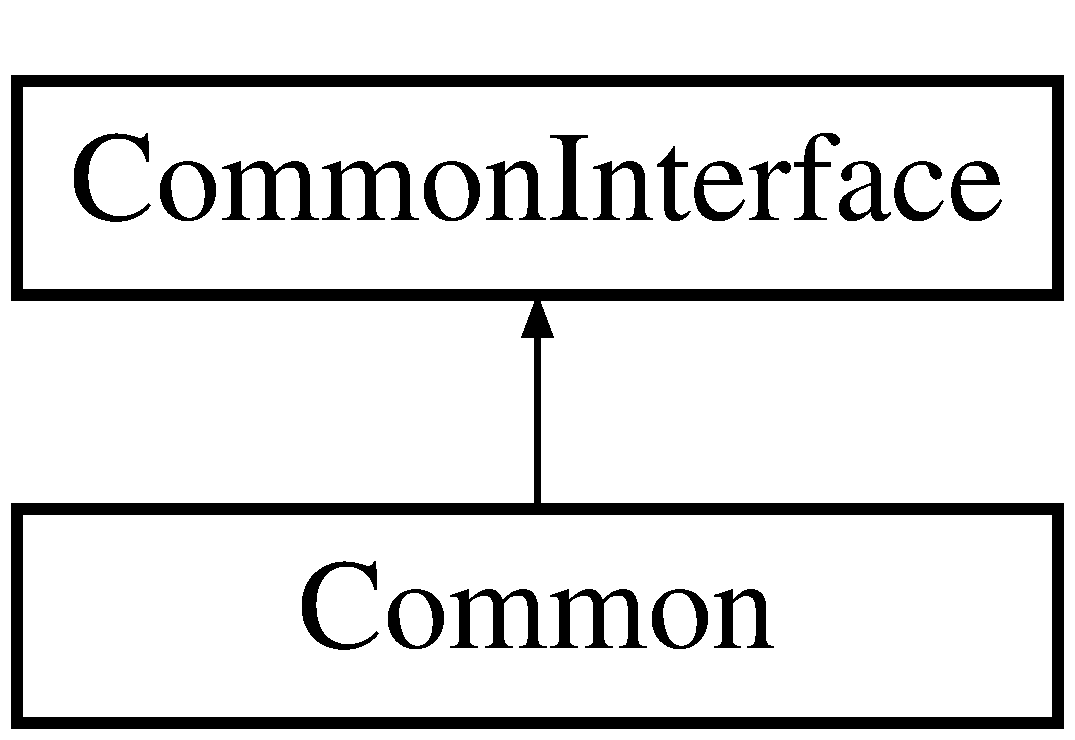
\includegraphics[height=2.000000cm]{class_common}
\end{center}
\end{figure}
\subsection*{Public Member Functions}
\begin{DoxyCompactItemize}
\item 
\hyperlink{class_common_a4a9e6769ab6c946d0895e8d987df1c10}{Common} (\$debug)
\item 
\hyperlink{class_common_a1b1bd9b3f45a5fbd2549355282cdc96f}{connect} (\$db)
\item 
\hyperlink{class_common_a57a9dbd1203cf7b3ef3c5ce40d4047cc}{execute\+Query} (\$sql, \$filename)
\end{DoxyCompactItemize}
\subsection*{Data Fields}
\begin{DoxyCompactItemize}
\item 
{\bfseries \$conn}\hypertarget{class_common_aa8a5a87b9c1a6a0819b88447cbe41877}{}\label{class_common_aa8a5a87b9c1a6a0819b88447cbe41877}

\item 
{\bfseries \$debug}\hypertarget{class_common_a85ae3e64cd40e9564adceb010085e9dd}{}\label{class_common_a85ae3e64cd40e9564adceb010085e9dd}

\item 
{\bfseries \$db} =\char`\"{}database.\+cse.\+tamu.\+edu\char`\"{}\hypertarget{class_common_a1fa3127fc82f96b1436d871ef02be319}{}\label{class_common_a1fa3127fc82f96b1436d871ef02be319}

\item 
{\bfseries \$dbname} =\char`\"{}jgwesterfield-\/Tamu\+Driver\char`\"{}\hypertarget{class_common_ac5111a571fffa2499732833bb7f0d8c1}{}\label{class_common_ac5111a571fffa2499732833bb7f0d8c1}

\item 
{\bfseries \$user} =\char`\"{}jgwesterfield\char`\"{}\hypertarget{class_common_a598ca4e71b15a1313ec95f0df1027ca5}{}\label{class_common_a598ca4e71b15a1313ec95f0df1027ca5}

\item 
{\bfseries \$pass} =\char`\"{}Whoop19!\char`\"{}\hypertarget{class_common_a12ec2780b52bd1c54d38c2f981c0349f}{}\label{class_common_a12ec2780b52bd1c54d38c2f981c0349f}

\end{DoxyCompactItemize}


\subsection{Detailed Description}
\hyperlink{class_common}{Common} is responsible for actually connecting to the My\+S\+QL database. The \hyperlink{class_common}{Common} class object must be created and the \hyperlink{class_common_a1b1bd9b3f45a5fbd2549355282cdc96f}{connect()} function run before any functions on the database can be performed. 

\subsection{Member Function Documentation}
\index{Common@{Common}!Common@{Common}}
\index{Common@{Common}!Common@{Common}}
\subsubsection[{\texorpdfstring{Common(\$debug)}{Common($debug)}}]{\setlength{\rightskip}{0pt plus 5cm}{\bf Common} (
\begin{DoxyParamCaption}
\item[{}]{\$debug}
\end{DoxyParamCaption}
)}\hypertarget{class_common_a4a9e6769ab6c946d0895e8d987df1c10}{}\label{class_common_a4a9e6769ab6c946d0895e8d987df1c10}
\hyperlink{class_common}{Common} constructor. 
\begin{DoxyParams}{Parameters}
{\em \$debug} & The constructor for the \hyperlink{class_common}{Common} class \\
\hline
\end{DoxyParams}


Implements \hyperlink{interface_common_interface_a4a9e6769ab6c946d0895e8d987df1c10}{Common\+Interface}.

\index{Common@{Common}!connect@{connect}}
\index{connect@{connect}!Common@{Common}}
\subsubsection[{\texorpdfstring{connect(\$db)}{connect($db)}}]{\setlength{\rightskip}{0pt plus 5cm}connect (
\begin{DoxyParamCaption}
\item[{}]{\$db}
\end{DoxyParamCaption}
)}\hypertarget{class_common_a1b1bd9b3f45a5fbd2549355282cdc96f}{}\label{class_common_a1b1bd9b3f45a5fbd2549355282cdc96f}

\begin{DoxyParams}{Parameters}
{\em \$db} & Uses the \$db class member functions to actually make the connection to the database \\
\hline
\end{DoxyParams}


Implements \hyperlink{interface_common_interface_a1b1bd9b3f45a5fbd2549355282cdc96f}{Common\+Interface}.

\index{Common@{Common}!execute\+Query@{execute\+Query}}
\index{execute\+Query@{execute\+Query}!Common@{Common}}
\subsubsection[{\texorpdfstring{execute\+Query(\$sql, \$filename)}{executeQuery($sql, $filename)}}]{\setlength{\rightskip}{0pt plus 5cm}execute\+Query (
\begin{DoxyParamCaption}
\item[{}]{\$sql, }
\item[{}]{\$filename}
\end{DoxyParamCaption}
)}\hypertarget{class_common_a57a9dbd1203cf7b3ef3c5ce40d4047cc}{}\label{class_common_a57a9dbd1203cf7b3ef3c5ce40d4047cc}

\begin{DoxyParams}{Parameters}
{\em \$sql} & \\
\hline
{\em \$filename} & \\
\hline
\end{DoxyParams}
\begin{DoxyReturn}{Returns}
mixed
\end{DoxyReturn}
Uses the sql statement that is passed in and executes the query

Example Code\+: ~\newline
 \$sql = \char`\"{}\+S\+E\+L\+E\+C\+T C\+O\+U\+N\+T(\+Walker\+Number) F\+R\+O\+M Walker\+Data\char`\"{}; ~\newline
 \$rs = \$this-\/$>$C\+O\+M\+M\+O\+N-\/$>$execute\+Query(\$sql, \$\+\_\+\+S\+E\+R\+V\+ER\mbox{[}\char`\"{}\+S\+C\+R\+I\+P\+T\+\_\+\+N\+A\+M\+E\char`\"{}\mbox{]}); ~\newline
 \$row = \$rs-\/$>$fetch(\+P\+D\+O\+::\+F\+E\+T\+C\+H\+\_\+\+A\+S\+S\+O\+C); ~\newline
 return (int)\$row\mbox{[}\textquotesingle{}C\+O\+U\+N\+T(\+Walker\+Number)\textquotesingle{}\mbox{]}; ~\newline
 

Implements \hyperlink{interface_common_interface_a57a9dbd1203cf7b3ef3c5ce40d4047cc}{Common\+Interface}.



The documentation for this class was generated from the following file\+:\begin{DoxyCompactItemize}
\item 
P\+H\+P Server Code/Common\+Methods.\+php\end{DoxyCompactItemize}

\hypertarget{interface_common_interface}{}\section{Common\+Interface Interface Reference}
\label{interface_common_interface}\index{Common\+Interface@{Common\+Interface}}


Interface to for the Common\+Methods.\+php file. Include this file in your code instead of the Common\+Methods.\+php file.  


Inheritance diagram for Common\+Interface\+:\begin{figure}[H]
\begin{center}
\leavevmode
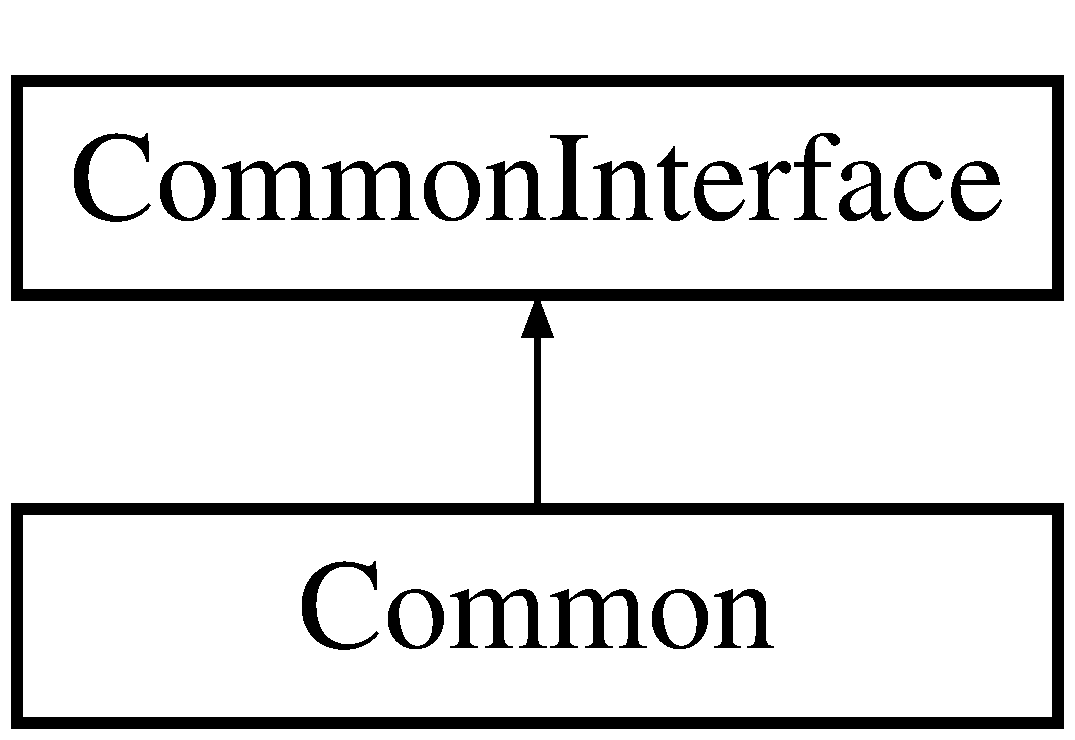
\includegraphics[height=2.000000cm]{interface_common_interface}
\end{center}
\end{figure}
\subsection*{Public Member Functions}
\begin{DoxyCompactItemize}
\item 
\hyperlink{interface_common_interface_a4a9e6769ab6c946d0895e8d987df1c10}{Common} (\$debug)
\item 
\hyperlink{interface_common_interface_a1b1bd9b3f45a5fbd2549355282cdc96f}{connect} (\$db)
\item 
\hyperlink{interface_common_interface_a57a9dbd1203cf7b3ef3c5ce40d4047cc}{execute\+Query} (\$sql, \$filename)
\end{DoxyCompactItemize}


\subsection{Detailed Description}
Interface to for the Common\+Methods.\+php file. Include this file in your code instead of the Common\+Methods.\+php file. 

\subsection{Member Function Documentation}
\index{Common\+Interface@{Common\+Interface}!Common@{Common}}
\index{Common@{Common}!Common\+Interface@{Common\+Interface}}
\subsubsection[{\texorpdfstring{Common(\$debug)}{Common($debug)}}]{\setlength{\rightskip}{0pt plus 5cm}{\bf Common} (
\begin{DoxyParamCaption}
\item[{}]{\$debug}
\end{DoxyParamCaption}
)}\hypertarget{interface_common_interface_a4a9e6769ab6c946d0895e8d987df1c10}{}\label{interface_common_interface_a4a9e6769ab6c946d0895e8d987df1c10}
\hyperlink{class_common}{Common} constructor. 
\begin{DoxyParams}{Parameters}
{\em \$debug} & The constructor for the \hyperlink{class_common}{Common} class \\
\hline
\end{DoxyParams}


Implemented in \hyperlink{class_common_a4a9e6769ab6c946d0895e8d987df1c10}{Common}.

\index{Common\+Interface@{Common\+Interface}!connect@{connect}}
\index{connect@{connect}!Common\+Interface@{Common\+Interface}}
\subsubsection[{\texorpdfstring{connect(\$db)}{connect($db)}}]{\setlength{\rightskip}{0pt plus 5cm}connect (
\begin{DoxyParamCaption}
\item[{}]{\$db}
\end{DoxyParamCaption}
)}\hypertarget{interface_common_interface_a1b1bd9b3f45a5fbd2549355282cdc96f}{}\label{interface_common_interface_a1b1bd9b3f45a5fbd2549355282cdc96f}

\begin{DoxyParams}{Parameters}
{\em \$db} & Uses the \$db class member functions to actually make the connection to the database \\
\hline
\end{DoxyParams}


Implemented in \hyperlink{class_common_a1b1bd9b3f45a5fbd2549355282cdc96f}{Common}.

\index{Common\+Interface@{Common\+Interface}!execute\+Query@{execute\+Query}}
\index{execute\+Query@{execute\+Query}!Common\+Interface@{Common\+Interface}}
\subsubsection[{\texorpdfstring{execute\+Query(\$sql, \$filename)}{executeQuery($sql, $filename)}}]{\setlength{\rightskip}{0pt plus 5cm}execute\+Query (
\begin{DoxyParamCaption}
\item[{}]{\$sql, }
\item[{}]{\$filename}
\end{DoxyParamCaption}
)}\hypertarget{interface_common_interface_a57a9dbd1203cf7b3ef3c5ce40d4047cc}{}\label{interface_common_interface_a57a9dbd1203cf7b3ef3c5ce40d4047cc}

\begin{DoxyParams}{Parameters}
{\em \$sql} & \\
\hline
{\em \$filename} & \\
\hline
\end{DoxyParams}
\begin{DoxyReturn}{Returns}
mixed
\end{DoxyReturn}
Uses the sql statement that is passed in and executes the query

Example Code\+: ~\newline
 \$sql = \char`\"{}\+S\+E\+L\+E\+C\+T C\+O\+U\+N\+T(\+Walker\+Number) F\+R\+O\+M Walker\+Data\char`\"{}; ~\newline
 \$rs = \$this-\/$>$C\+O\+M\+M\+O\+N-\/$>$execute\+Query(\$sql, \$\+\_\+\+S\+E\+R\+V\+ER\mbox{[}\char`\"{}\+S\+C\+R\+I\+P\+T\+\_\+\+N\+A\+M\+E\char`\"{}\mbox{]}); ~\newline
 \$row = \$rs-\/$>$fetch(\+P\+D\+O\+::\+F\+E\+T\+C\+H\+\_\+\+A\+S\+S\+O\+C); ~\newline
 return (int)\$row\mbox{[}\textquotesingle{}C\+O\+U\+N\+T(\+Walker\+Number)\textquotesingle{}\mbox{]}; ~\newline
 

Implemented in \hyperlink{class_common_a57a9dbd1203cf7b3ef3c5ce40d4047cc}{Common}.



The documentation for this interface was generated from the following file\+:\begin{DoxyCompactItemize}
\item 
P\+H\+P Server Code/Common\+Interface.\+php\end{DoxyCompactItemize}

\hypertarget{class_p_h_pto_s_q_l}{}\section{P\+H\+Pto\+S\+QL Class Reference}
\label{class_p_h_pto_s_q_l}\index{P\+H\+Pto\+S\+QL@{P\+H\+Pto\+S\+QL}}
Inheritance diagram for P\+H\+Pto\+S\+QL\+:\begin{figure}[H]
\begin{center}
\leavevmode
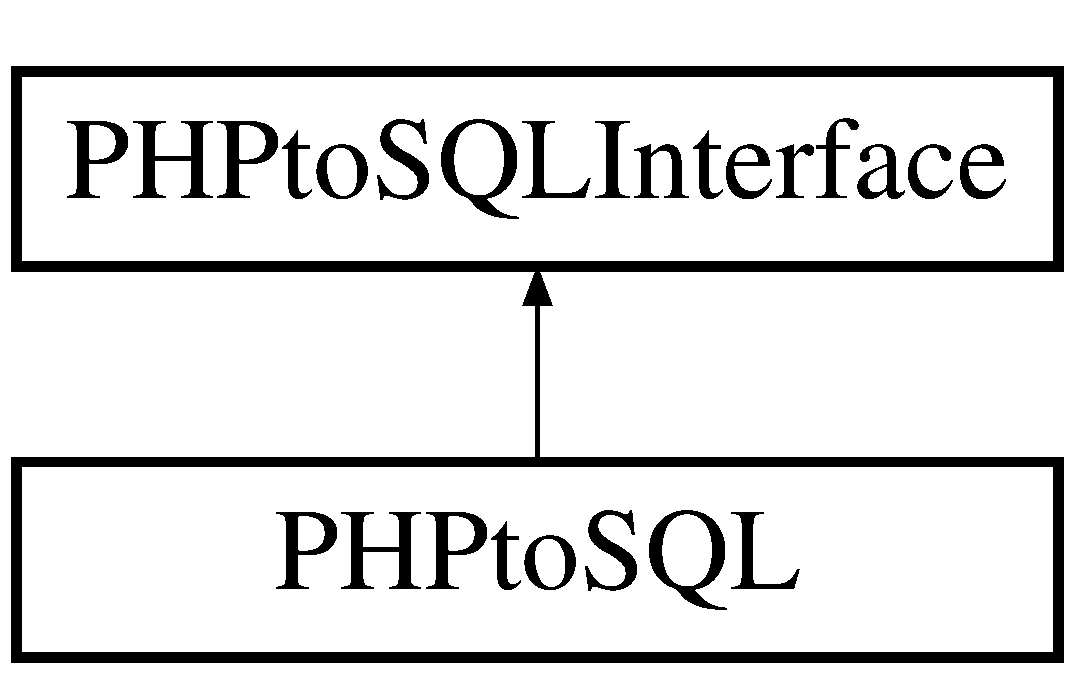
\includegraphics[height=2.000000cm]{class_p_h_pto_s_q_l}
\end{center}
\end{figure}
\subsection*{Public Member Functions}
\begin{DoxyCompactItemize}
\item 
\hyperlink{class_p_h_pto_s_q_l_a800f8efee13692788b13ee57c5960092}{\+\_\+\+\_\+construct} (\$db)
\item 
\hyperlink{class_p_h_pto_s_q_l_a421831a265621325e1fdd19aace0c758}{\+\_\+\+\_\+destruct} ()
\item 
\hyperlink{class_p_h_pto_s_q_l_a6e6deaf037e5413c56743ab1985fc0b6}{get\+Num\+Cars\+This\+Week} (\$location\+Choice)
\item 
\hyperlink{class_p_h_pto_s_q_l_a88bd9a6c7f64a8f733270a7134204ebb}{get\+Traffic\+By\+Year} (\$year, \$location\+Choice)
\item 
\hyperlink{class_p_h_pto_s_q_l_a2389b15a72a087f39f462b1ff8f8ef95}{get\+Traffic\+By\+Month} (\$year, \$month, \$location\+Choice)
\item 
\hyperlink{class_p_h_pto_s_q_l_a6278f024da07a6ff95ffcf3efc6c0c5d}{get\+Traffic\+By\+Day} (\$year, \$month, \$day, \$location\+Choice)
\item 
\hyperlink{class_p_h_pto_s_q_l_ac91d0c56506620188f25007d30f1e8d0}{get\+Traffic\+Time\+Range} (\$year1, \$month1, \$day1, \$year2, \$month2, \$day2, \$location\+Choice)
\item 
\hyperlink{class_p_h_pto_s_q_l_a64377368eb86a5a874483663c7da1407}{get\+List\+Of\+Locations} ()
\item 
\hyperlink{class_p_h_pto_s_q_l_acc7b884d5cfc62ca661996820eebbba2}{Get\+Minimum\+Count\+In\+Hour} (\$count\+By\+Hour, \$date\+By\+Hour)
\item 
\hyperlink{class_p_h_pto_s_q_l_a59876f14f59f0b3321ae144eb0987692}{Get\+Median\+Count\+In\+Hour} (\$count\+By\+Hour, \$date\+By\+Hour)
\item 
\hyperlink{class_p_h_pto_s_q_l_ab4dfd011e2c8436c0284c99573d30d4a}{Get\+Maximum\+Count\+In\+Hour} (\$count\+By\+Hour, \$date\+By\+Hour)
\item 
\hyperlink{class_p_h_pto_s_q_l_a085d2dda8ee0aa89eba99f4b475851d1}{Get\+Average\+Count\+In\+Hour} (\$count\+By\+Hour)
\item 
\hyperlink{class_p_h_pto_s_q_l_ac5a84f4e20620ec0cfac496528ce01ec}{Execute\+Query} (\$Time1, \$Time2, \$C\+O\+M\+M\+ON)
\begin{DoxyCompactList}\small\item\em A function to execute a query of correct My\+S\+QL syntax for the specified instance of the database within a certain time range. \end{DoxyCompactList}\item 
\hyperlink{class_p_h_pto_s_q_l_adbaa8f880037cb88ee1f527f6c0971b2}{Convert\+Time} (\$Time)
\item 
\hyperlink{class_p_h_pto_s_q_l_a01acbca2f4fed77736c1c498fb57583c}{Print\+Results} (\$results)
\item 
\hyperlink{class_p_h_pto_s_q_l_a8fcdf2951d5159f94775133b11c29328}{Group\+Results\+By\+Hour} (\$results)
\item 
\hyperlink{class_p_h_pto_s_q_l_a939709f50283d3d5e8297fb0f608acf4}{Reformat\+Date} (\$date)
\item 
{\bfseries Get\+Dates\+Of\+Past\+Week} ()\hypertarget{class_p_h_pto_s_q_l_af531a42121fec567ccbf5c13ce3379fe}{}\label{class_p_h_pto_s_q_l_af531a42121fec567ccbf5c13ce3379fe}

\item 
{\bfseries Get\+Traffic\+Count\+For\+Dates} (\$results, \$dates)\hypertarget{class_p_h_pto_s_q_l_ab232e3d0dd7c916311edaeba9c2e223f}{}\label{class_p_h_pto_s_q_l_ab232e3d0dd7c916311edaeba9c2e223f}

\end{DoxyCompactItemize}


\subsection{Constructor \& Destructor Documentation}
\index{P\+H\+Pto\+S\+QL@{P\+H\+Pto\+S\+QL}!\+\_\+\+\_\+construct@{\+\_\+\+\_\+construct}}
\index{\+\_\+\+\_\+construct@{\+\_\+\+\_\+construct}!P\+H\+Pto\+S\+QL@{P\+H\+Pto\+S\+QL}}
\subsubsection[{\texorpdfstring{\+\_\+\+\_\+construct(\$db)}{__construct($db)}}]{\setlength{\rightskip}{0pt plus 5cm}\+\_\+\+\_\+construct (
\begin{DoxyParamCaption}
\item[{}]{\$db}
\end{DoxyParamCaption}
)}\hypertarget{class_p_h_pto_s_q_l_a800f8efee13692788b13ee57c5960092}{}\label{class_p_h_pto_s_q_l_a800f8efee13692788b13ee57c5960092}
D\+B\+A\+PI constructor. 
\begin{DoxyParams}{Parameters}
{\em \$db} & Mostly sets up the dates in this object. Also sets the timezone to our timezone. \\
\hline
\end{DoxyParams}


Implements \hyperlink{interface_p_h_pto_s_q_l_interface_a800f8efee13692788b13ee57c5960092}{P\+H\+Pto\+S\+Q\+L\+Interface}.

\index{P\+H\+Pto\+S\+QL@{P\+H\+Pto\+S\+QL}!\+\_\+\+\_\+destruct@{\+\_\+\+\_\+destruct}}
\index{\+\_\+\+\_\+destruct@{\+\_\+\+\_\+destruct}!P\+H\+Pto\+S\+QL@{P\+H\+Pto\+S\+QL}}
\subsubsection[{\texorpdfstring{\+\_\+\+\_\+destruct()}{__destruct()}}]{\setlength{\rightskip}{0pt plus 5cm}\+\_\+\+\_\+destruct (
\begin{DoxyParamCaption}
{}
\end{DoxyParamCaption}
)}\hypertarget{class_p_h_pto_s_q_l_a421831a265621325e1fdd19aace0c758}{}\label{class_p_h_pto_s_q_l_a421831a265621325e1fdd19aace0c758}
Class destructor 

Implements \hyperlink{interface_p_h_pto_s_q_l_interface_a421831a265621325e1fdd19aace0c758}{P\+H\+Pto\+S\+Q\+L\+Interface}.



\subsection{Member Function Documentation}
\index{P\+H\+Pto\+S\+QL@{P\+H\+Pto\+S\+QL}!Convert\+Time@{Convert\+Time}}
\index{Convert\+Time@{Convert\+Time}!P\+H\+Pto\+S\+QL@{P\+H\+Pto\+S\+QL}}
\subsubsection[{\texorpdfstring{Convert\+Time(\$\+Time)}{ConvertTime($Time)}}]{\setlength{\rightskip}{0pt plus 5cm}Convert\+Time (
\begin{DoxyParamCaption}
\item[{}]{\$\+Time}
\end{DoxyParamCaption}
)}\hypertarget{class_p_h_pto_s_q_l_adbaa8f880037cb88ee1f527f6c0971b2}{}\label{class_p_h_pto_s_q_l_adbaa8f880037cb88ee1f527f6c0971b2}

\begin{DoxyParams}{Parameters}
{\em \$\+Time} & -\/ timestamp of the format ‘\+Y\+Y\+Y\+Y-\/\+M\+M-\/\+D\+D\+T\+HH\+:M\+M’. \\
\hline
\end{DoxyParams}
\begin{DoxyReturn}{Returns}
string -\/ which is of the form ‘\+Y\+Y\+Y\+Y-\/\+M\+M-\/\+DD H\+H\+:\+MM\+:00’.
\end{DoxyReturn}
Converts a time of a certain format to that of another. 

Implements \hyperlink{interface_p_h_pto_s_q_l_interface_adbaa8f880037cb88ee1f527f6c0971b2}{P\+H\+Pto\+S\+Q\+L\+Interface}.

\index{P\+H\+Pto\+S\+QL@{P\+H\+Pto\+S\+QL}!Execute\+Query@{Execute\+Query}}
\index{Execute\+Query@{Execute\+Query}!P\+H\+Pto\+S\+QL@{P\+H\+Pto\+S\+QL}}
\subsubsection[{\texorpdfstring{Execute\+Query(\$\+Time1, \$\+Time2, \$\+C\+O\+M\+M\+O\+N)}{ExecuteQuery($Time1, $Time2, $COMMON)}}]{\setlength{\rightskip}{0pt plus 5cm}Execute\+Query (
\begin{DoxyParamCaption}
\item[{}]{\$\+Time1, }
\item[{}]{\$\+Time2, }
\item[{}]{\$\+C\+O\+M\+M\+ON}
\end{DoxyParamCaption}
)}\hypertarget{class_p_h_pto_s_q_l_ac5a84f4e20620ec0cfac496528ce01ec}{}\label{class_p_h_pto_s_q_l_ac5a84f4e20620ec0cfac496528ce01ec}


A function to execute a query of correct My\+S\+QL syntax for the specified instance of the database within a certain time range. 


\begin{DoxyParams}{Parameters}
{\em \$\+Time1} & -\/ First timestamp of the format ‘\+Y\+Y\+Y\+Y-\/\+M\+M-\/\+DD H\+H\+:\+MM\+:00’ \\
\hline
{\em \$\+Time2} & -\/ Second timestamp of the format ‘\+Y\+Y\+Y\+Y-\/\+M\+M-\/\+DD H\+H\+:\+MM\+:00’. \\
\hline
{\em \$\+C\+O\+M\+M\+ON} & -\/ common instance that connects to the database. \\
\hline
\end{DoxyParams}
\begin{DoxyReturn}{Returns}
array -\/ all of the resulting data (in rows) returned from the query.
\end{DoxyReturn}
Usage\+: ~\newline
 \$\+Time1 = \$\+\_\+\+P\+O\+ST\mbox{[}\char`\"{}\+Time1\char`\"{}\mbox{]}; ~\newline
 \$\+Time2 = \$\+\_\+\+P\+O\+ST\mbox{[}\char`\"{}\+Time2\char`\"{}\mbox{]}; ~\newline
 // Convert input times into the correct Timestamp format ~\newline
 \$time1\+Format = Convert\+Time(\$\+Time1); ~\newline
 \$time2\+Format = Convert\+Time(\$\+Time2); ~\newline
 // Create a new \hyperlink{class_common}{Common} instance to connect to the database ~\newline
 \$debug = false; ~\newline
 \$\+C\+O\+M\+M\+ON = new \hyperlink{class_common}{Common}(\$debug); ~\newline
 // Execute query and fetch the results ~\newline
 \$results = Execute\+Query(\$time1\+Format, \$time2\+Format, \$\+C\+O\+M\+M\+ON); ~\newline
 

Implements \hyperlink{interface_p_h_pto_s_q_l_interface_ac5a84f4e20620ec0cfac496528ce01ec}{P\+H\+Pto\+S\+Q\+L\+Interface}.

\index{P\+H\+Pto\+S\+QL@{P\+H\+Pto\+S\+QL}!Get\+Average\+Count\+In\+Hour@{Get\+Average\+Count\+In\+Hour}}
\index{Get\+Average\+Count\+In\+Hour@{Get\+Average\+Count\+In\+Hour}!P\+H\+Pto\+S\+QL@{P\+H\+Pto\+S\+QL}}
\subsubsection[{\texorpdfstring{Get\+Average\+Count\+In\+Hour(\$count\+By\+Hour)}{GetAverageCountInHour($countByHour)}}]{\setlength{\rightskip}{0pt plus 5cm}Get\+Average\+Count\+In\+Hour (
\begin{DoxyParamCaption}
\item[{}]{\$count\+By\+Hour}
\end{DoxyParamCaption}
)}\hypertarget{class_p_h_pto_s_q_l_a085d2dda8ee0aa89eba99f4b475851d1}{}\label{class_p_h_pto_s_q_l_a085d2dda8ee0aa89eba99f4b475851d1}

\begin{DoxyParams}{Parameters}
{\em \$count\+By\+Hour} & -\/ the array of counts by hour returned from Group\+Results\+By\+Hour. \\
\hline
\end{DoxyParams}
\begin{DoxyReturn}{Returns}
integer -\/ Returns the average number of people recorded in an hour of the specific time range.
\end{DoxyReturn}
Finds average number of people counted during an hour in a specific time range. 

Implements \hyperlink{interface_p_h_pto_s_q_l_interface_a085d2dda8ee0aa89eba99f4b475851d1}{P\+H\+Pto\+S\+Q\+L\+Interface}.

\index{P\+H\+Pto\+S\+QL@{P\+H\+Pto\+S\+QL}!get\+List\+Of\+Locations@{get\+List\+Of\+Locations}}
\index{get\+List\+Of\+Locations@{get\+List\+Of\+Locations}!P\+H\+Pto\+S\+QL@{P\+H\+Pto\+S\+QL}}
\subsubsection[{\texorpdfstring{get\+List\+Of\+Locations()}{getListOfLocations()}}]{\setlength{\rightskip}{0pt plus 5cm}get\+List\+Of\+Locations (
\begin{DoxyParamCaption}
{}
\end{DoxyParamCaption}
)}\hypertarget{class_p_h_pto_s_q_l_a64377368eb86a5a874483663c7da1407}{}\label{class_p_h_pto_s_q_l_a64377368eb86a5a874483663c7da1407}
\begin{DoxyReturn}{Returns}
array of strings
\end{DoxyReturn}
Will return the names of all different locations (parking lots) that are being recorded in the database 

Implements \hyperlink{interface_p_h_pto_s_q_l_interface_a64377368eb86a5a874483663c7da1407}{P\+H\+Pto\+S\+Q\+L\+Interface}.

\index{P\+H\+Pto\+S\+QL@{P\+H\+Pto\+S\+QL}!Get\+Maximum\+Count\+In\+Hour@{Get\+Maximum\+Count\+In\+Hour}}
\index{Get\+Maximum\+Count\+In\+Hour@{Get\+Maximum\+Count\+In\+Hour}!P\+H\+Pto\+S\+QL@{P\+H\+Pto\+S\+QL}}
\subsubsection[{\texorpdfstring{Get\+Maximum\+Count\+In\+Hour(\$count\+By\+Hour, \$date\+By\+Hour)}{GetMaximumCountInHour($countByHour, $dateByHour)}}]{\setlength{\rightskip}{0pt plus 5cm}Get\+Maximum\+Count\+In\+Hour (
\begin{DoxyParamCaption}
\item[{}]{\$count\+By\+Hour, }
\item[{}]{\$date\+By\+Hour}
\end{DoxyParamCaption}
)}\hypertarget{class_p_h_pto_s_q_l_ab4dfd011e2c8436c0284c99573d30d4a}{}\label{class_p_h_pto_s_q_l_ab4dfd011e2c8436c0284c99573d30d4a}

\begin{DoxyParams}{Parameters}
{\em \$count\+By\+Hour} & -\/ the array of counts by hour returned from Group\+Results\+By\+Hour. \\
\hline
{\em \$date\+By\+Hour} & -\/ the corresponding array of dates sorted by hour returned from Group\+Results\+By\+Hour. \\
\hline
\end{DoxyParams}
\begin{DoxyReturn}{Returns}
2 arrays -\/ Returns an array containing (1) the maximum count within an hour and (2) the corresponding time for which the count was recorded.
\end{DoxyReturn}
Finds the maximum count for an hour in a specific time range. 

Implements \hyperlink{interface_p_h_pto_s_q_l_interface_ab4dfd011e2c8436c0284c99573d30d4a}{P\+H\+Pto\+S\+Q\+L\+Interface}.

\index{P\+H\+Pto\+S\+QL@{P\+H\+Pto\+S\+QL}!Get\+Median\+Count\+In\+Hour@{Get\+Median\+Count\+In\+Hour}}
\index{Get\+Median\+Count\+In\+Hour@{Get\+Median\+Count\+In\+Hour}!P\+H\+Pto\+S\+QL@{P\+H\+Pto\+S\+QL}}
\subsubsection[{\texorpdfstring{Get\+Median\+Count\+In\+Hour(\$count\+By\+Hour, \$date\+By\+Hour)}{GetMedianCountInHour($countByHour, $dateByHour)}}]{\setlength{\rightskip}{0pt plus 5cm}Get\+Median\+Count\+In\+Hour (
\begin{DoxyParamCaption}
\item[{}]{\$count\+By\+Hour, }
\item[{}]{\$date\+By\+Hour}
\end{DoxyParamCaption}
)}\hypertarget{class_p_h_pto_s_q_l_a59876f14f59f0b3321ae144eb0987692}{}\label{class_p_h_pto_s_q_l_a59876f14f59f0b3321ae144eb0987692}

\begin{DoxyParams}{Parameters}
{\em \$count\+By\+Hour} & -\/ the array of counts by hour returned from Group\+Results\+By\+Hour. \\
\hline
{\em \$date\+By\+Hour} & -\/ the corresponding array of dates sorted by hour returned from Group\+Results\+By\+Hour. \\
\hline
\end{DoxyParams}
\begin{DoxyReturn}{Returns}
array -\/ Returns an array containing (1) the median count within an hour and (2) the corresponding time for which the count was recorded.
\end{DoxyReturn}
Finds the median count for an hour in a specific time range. 

Implements \hyperlink{interface_p_h_pto_s_q_l_interface_a59876f14f59f0b3321ae144eb0987692}{P\+H\+Pto\+S\+Q\+L\+Interface}.

\index{P\+H\+Pto\+S\+QL@{P\+H\+Pto\+S\+QL}!Get\+Minimum\+Count\+In\+Hour@{Get\+Minimum\+Count\+In\+Hour}}
\index{Get\+Minimum\+Count\+In\+Hour@{Get\+Minimum\+Count\+In\+Hour}!P\+H\+Pto\+S\+QL@{P\+H\+Pto\+S\+QL}}
\subsubsection[{\texorpdfstring{Get\+Minimum\+Count\+In\+Hour(\$count\+By\+Hour, \$date\+By\+Hour)}{GetMinimumCountInHour($countByHour, $dateByHour)}}]{\setlength{\rightskip}{0pt plus 5cm}Get\+Minimum\+Count\+In\+Hour (
\begin{DoxyParamCaption}
\item[{}]{\$count\+By\+Hour, }
\item[{}]{\$date\+By\+Hour}
\end{DoxyParamCaption}
)}\hypertarget{class_p_h_pto_s_q_l_acc7b884d5cfc62ca661996820eebbba2}{}\label{class_p_h_pto_s_q_l_acc7b884d5cfc62ca661996820eebbba2}

\begin{DoxyParams}{Parameters}
{\em \$count\+By\+Hour} & -\/ the corresponding array of dates sorted by hour returned from Group\+Results\+By\+Hour. \\
\hline
{\em \$date\+By\+Hour} & -\/ the array of counts by hour returned from Group\+Results\+By\+Hour. \\
\hline
\end{DoxyParams}
\begin{DoxyReturn}{Returns}
Returns an array containing (1) the minimum count within an hour and (2) the corresponding time for which the count was recorded.
\end{DoxyReturn}
Finds the minimum count for an hour in a specific time range. 

Implements \hyperlink{interface_p_h_pto_s_q_l_interface_acc7b884d5cfc62ca661996820eebbba2}{P\+H\+Pto\+S\+Q\+L\+Interface}.

\index{P\+H\+Pto\+S\+QL@{P\+H\+Pto\+S\+QL}!get\+Num\+Cars\+This\+Week@{get\+Num\+Cars\+This\+Week}}
\index{get\+Num\+Cars\+This\+Week@{get\+Num\+Cars\+This\+Week}!P\+H\+Pto\+S\+QL@{P\+H\+Pto\+S\+QL}}
\subsubsection[{\texorpdfstring{get\+Num\+Cars\+This\+Week(\$location\+Choice)}{getNumCarsThisWeek($locationChoice)}}]{\setlength{\rightskip}{0pt plus 5cm}get\+Num\+Cars\+This\+Week (
\begin{DoxyParamCaption}
\item[{}]{\$location\+Choice}
\end{DoxyParamCaption}
)}\hypertarget{class_p_h_pto_s_q_l_a6e6deaf037e5413c56743ab1985fc0b6}{}\label{class_p_h_pto_s_q_l_a6e6deaf037e5413c56743ab1985fc0b6}
\begin{DoxyReturn}{Returns}
int
\end{DoxyReturn}
Gets the number of cars in the last week starting from today Usage\+: \$num\+Cars = get\+Num\+Cars\+This\+Week(\char`\"{}lot35\char`\"{}); for Lot 35 

Implements \hyperlink{interface_p_h_pto_s_q_l_interface_a6e6deaf037e5413c56743ab1985fc0b6}{P\+H\+Pto\+S\+Q\+L\+Interface}.

\index{P\+H\+Pto\+S\+QL@{P\+H\+Pto\+S\+QL}!get\+Traffic\+By\+Day@{get\+Traffic\+By\+Day}}
\index{get\+Traffic\+By\+Day@{get\+Traffic\+By\+Day}!P\+H\+Pto\+S\+QL@{P\+H\+Pto\+S\+QL}}
\subsubsection[{\texorpdfstring{get\+Traffic\+By\+Day(\$year, \$month, \$day, \$location\+Choice)}{getTrafficByDay($year, $month, $day, $locationChoice)}}]{\setlength{\rightskip}{0pt plus 5cm}get\+Traffic\+By\+Day (
\begin{DoxyParamCaption}
\item[{}]{\$year, }
\item[{}]{\$month, }
\item[{}]{\$day, }
\item[{}]{\$location\+Choice}
\end{DoxyParamCaption}
)}\hypertarget{class_p_h_pto_s_q_l_a6278f024da07a6ff95ffcf3efc6c0c5d}{}\label{class_p_h_pto_s_q_l_a6278f024da07a6ff95ffcf3efc6c0c5d}

\begin{DoxyParams}{Parameters}
{\em \$year} & \\
\hline
{\em \$month} & \\
\hline
{\em \$day} & \\
\hline
{\em \$location\+Choice} & \\
\hline
\end{DoxyParams}
\begin{DoxyReturn}{Returns}
int array -\/ length 24 array with the traffic number for each our of the day
\end{DoxyReturn}
Gets the traffic for each hour and returns it in a 24 element array.

Usage\+: $<$ \$day\+Array = get\+Traffic\+By\+Day(2018, 2, 15, \char`\"{}lot35\char`\"{});$>$ for Febraury 15, 2018 for Lot 35 output the times to see if I overshot how many times to iterate 

Implements \hyperlink{interface_p_h_pto_s_q_l_interface_a6278f024da07a6ff95ffcf3efc6c0c5d}{P\+H\+Pto\+S\+Q\+L\+Interface}.

\index{P\+H\+Pto\+S\+QL@{P\+H\+Pto\+S\+QL}!get\+Traffic\+By\+Month@{get\+Traffic\+By\+Month}}
\index{get\+Traffic\+By\+Month@{get\+Traffic\+By\+Month}!P\+H\+Pto\+S\+QL@{P\+H\+Pto\+S\+QL}}
\subsubsection[{\texorpdfstring{get\+Traffic\+By\+Month(\$year, \$month, \$location\+Choice)}{getTrafficByMonth($year, $month, $locationChoice)}}]{\setlength{\rightskip}{0pt plus 5cm}get\+Traffic\+By\+Month (
\begin{DoxyParamCaption}
\item[{}]{\$year, }
\item[{}]{\$month, }
\item[{}]{\$location\+Choice}
\end{DoxyParamCaption}
)}\hypertarget{class_p_h_pto_s_q_l_a2389b15a72a087f39f462b1ff8f8ef95}{}\label{class_p_h_pto_s_q_l_a2389b15a72a087f39f462b1ff8f8ef95}

\begin{DoxyParams}{Parameters}
{\em \$year} & \\
\hline
{\em \$month} & \\
\hline
{\em \$location\+Choice} & \\
\hline
\end{DoxyParams}
\begin{DoxyReturn}{Returns}
int array -\/ array with the traffic number for each day of the specified month
\end{DoxyReturn}
Gets the traffic for each day during the specified month of the specified year

Usage\+: \$month\+Array = get\+Traffic\+By\+Month(2018, 2, \char`\"{}lot35\char`\"{}); // for February 2018 for Lot 35 

Implements \hyperlink{interface_p_h_pto_s_q_l_interface_a2389b15a72a087f39f462b1ff8f8ef95}{P\+H\+Pto\+S\+Q\+L\+Interface}.

\index{P\+H\+Pto\+S\+QL@{P\+H\+Pto\+S\+QL}!get\+Traffic\+By\+Year@{get\+Traffic\+By\+Year}}
\index{get\+Traffic\+By\+Year@{get\+Traffic\+By\+Year}!P\+H\+Pto\+S\+QL@{P\+H\+Pto\+S\+QL}}
\subsubsection[{\texorpdfstring{get\+Traffic\+By\+Year(\$year, \$location\+Choice)}{getTrafficByYear($year, $locationChoice)}}]{\setlength{\rightskip}{0pt plus 5cm}get\+Traffic\+By\+Year (
\begin{DoxyParamCaption}
\item[{}]{\$year, }
\item[{}]{\$location\+Choice}
\end{DoxyParamCaption}
)}\hypertarget{class_p_h_pto_s_q_l_a88bd9a6c7f64a8f733270a7134204ebb}{}\label{class_p_h_pto_s_q_l_a88bd9a6c7f64a8f733270a7134204ebb}

\begin{DoxyParams}{Parameters}
{\em \$year} & \\
\hline
{\em \$location\+Choice} & -\/ string for the lot you want to put in \\
\hline
\end{DoxyParams}
\begin{DoxyReturn}{Returns}
int array -\/ a length 12 array where each element is the number of cars that passed through for that month. If there were 8 cars that passed through in April, the element at index 3 would be 8
\end{DoxyReturn}
Gives the traffic for each month in an array for the specified year passed in.

Usage\+: \$year\+Array = get\+Traffic\+By\+Year(2018, \char`\"{}lot35\char`\"{}); for 2018 for Lot 35 

Implements \hyperlink{interface_p_h_pto_s_q_l_interface_a88bd9a6c7f64a8f733270a7134204ebb}{P\+H\+Pto\+S\+Q\+L\+Interface}.

\index{P\+H\+Pto\+S\+QL@{P\+H\+Pto\+S\+QL}!get\+Traffic\+Time\+Range@{get\+Traffic\+Time\+Range}}
\index{get\+Traffic\+Time\+Range@{get\+Traffic\+Time\+Range}!P\+H\+Pto\+S\+QL@{P\+H\+Pto\+S\+QL}}
\subsubsection[{\texorpdfstring{get\+Traffic\+Time\+Range(\$year1, \$month1, \$day1, \$year2, \$month2, \$day2, \$location\+Choice)}{getTrafficTimeRange($year1, $month1, $day1, $year2, $month2, $day2, $locationChoice)}}]{\setlength{\rightskip}{0pt plus 5cm}get\+Traffic\+Time\+Range (
\begin{DoxyParamCaption}
\item[{}]{\$year1, }
\item[{}]{\$month1, }
\item[{}]{\$day1, }
\item[{}]{\$year2, }
\item[{}]{\$month2, }
\item[{}]{\$day2, }
\item[{}]{\$location\+Choice}
\end{DoxyParamCaption}
)}\hypertarget{class_p_h_pto_s_q_l_ac91d0c56506620188f25007d30f1e8d0}{}\label{class_p_h_pto_s_q_l_ac91d0c56506620188f25007d30f1e8d0}

\begin{DoxyParams}{Parameters}
{\em \$year1} & \\
\hline
{\em \$month1} & \\
\hline
{\em \$day1} & \\
\hline
{\em \$year2} & \\
\hline
{\em \$month2} & \\
\hline
{\em \$day2} & \\
\hline
{\em \$location\+Choice} & \\
\hline
\end{DoxyParams}
\begin{DoxyReturn}{Returns}
integer -\/ the number of cars in the time range
\end{DoxyReturn}
Takes in a date range (start and end date) and counts the number of cars in the given range

Usage\+: \$traffic\+In\+Range = get\+Traffic\+Time\+Range(2018, 2, 15, 2018, 2, 28, \char`\"{}lot35\char`\"{}); for number of cars between 2/15/2018 and 2/28/2018 for Lot 35 

Implements \hyperlink{interface_p_h_pto_s_q_l_interface_ac91d0c56506620188f25007d30f1e8d0}{P\+H\+Pto\+S\+Q\+L\+Interface}.

\index{P\+H\+Pto\+S\+QL@{P\+H\+Pto\+S\+QL}!Group\+Results\+By\+Hour@{Group\+Results\+By\+Hour}}
\index{Group\+Results\+By\+Hour@{Group\+Results\+By\+Hour}!P\+H\+Pto\+S\+QL@{P\+H\+Pto\+S\+QL}}
\subsubsection[{\texorpdfstring{Group\+Results\+By\+Hour(\$results)}{GroupResultsByHour($results)}}]{\setlength{\rightskip}{0pt plus 5cm}Group\+Results\+By\+Hour (
\begin{DoxyParamCaption}
\item[{}]{\$results}
\end{DoxyParamCaption}
)}\hypertarget{class_p_h_pto_s_q_l_a8fcdf2951d5159f94775133b11c29328}{}\label{class_p_h_pto_s_q_l_a8fcdf2951d5159f94775133b11c29328}

\begin{DoxyParams}{Parameters}
{\em \$results} & -\/ the results returned from a query, specifically from the function, \hyperlink{class_p_h_pto_s_q_l_ac5a84f4e20620ec0cfac496528ce01ec}{Execute\+Query()}. \\
\hline
\end{DoxyParams}
\begin{DoxyReturn}{Returns}
array -\/ Returns an array containing (1) an array of the dates within the results, grouped by hour, and (2) an array containing the counts for each corresponding hour of the dates array.
\end{DoxyReturn}
Groups the results of a query by hour and counts the number of results within each hour of the time range. 

Implements \hyperlink{interface_p_h_pto_s_q_l_interface_a8fcdf2951d5159f94775133b11c29328}{P\+H\+Pto\+S\+Q\+L\+Interface}.

\index{P\+H\+Pto\+S\+QL@{P\+H\+Pto\+S\+QL}!Print\+Results@{Print\+Results}}
\index{Print\+Results@{Print\+Results}!P\+H\+Pto\+S\+QL@{P\+H\+Pto\+S\+QL}}
\subsubsection[{\texorpdfstring{Print\+Results(\$results)}{PrintResults($results)}}]{\setlength{\rightskip}{0pt plus 5cm}Print\+Results (
\begin{DoxyParamCaption}
\item[{}]{\$results}
\end{DoxyParamCaption}
)}\hypertarget{class_p_h_pto_s_q_l_a01acbca2f4fed77736c1c498fb57583c}{}\label{class_p_h_pto_s_q_l_a01acbca2f4fed77736c1c498fb57583c}

\begin{DoxyParams}{Parameters}
{\em \$results} & -\/ the results returned from a query, specifically from the function, \hyperlink{class_p_h_pto_s_q_l_ac5a84f4e20620ec0cfac496528ce01ec}{Execute\+Query()} \\
\hline
\end{DoxyParams}
\begin{DoxyReturn}{Returns}
void -\/ returns echo’s html code to return rows with an entry number and the timestamp for it
\end{DoxyReturn}
Print\+Results is a function used to print the results of a query. 

Implements \hyperlink{interface_p_h_pto_s_q_l_interface_a01acbca2f4fed77736c1c498fb57583c}{P\+H\+Pto\+S\+Q\+L\+Interface}.

\index{P\+H\+Pto\+S\+QL@{P\+H\+Pto\+S\+QL}!Reformat\+Date@{Reformat\+Date}}
\index{Reformat\+Date@{Reformat\+Date}!P\+H\+Pto\+S\+QL@{P\+H\+Pto\+S\+QL}}
\subsubsection[{\texorpdfstring{Reformat\+Date(\$date)}{ReformatDate($date)}}]{\setlength{\rightskip}{0pt plus 5cm}Reformat\+Date (
\begin{DoxyParamCaption}
\item[{}]{\$date}
\end{DoxyParamCaption}
)}\hypertarget{class_p_h_pto_s_q_l_a939709f50283d3d5e8297fb0f608acf4}{}\label{class_p_h_pto_s_q_l_a939709f50283d3d5e8297fb0f608acf4}

\begin{DoxyParams}{Parameters}
{\em \$date} & -\/ A date in format \char`\"{}\+Y\+Y\+Y\+Y-\/\+M\+M-\/\+D\+D H\+H\char`\"{} where HH ranges from 00 to 23. \\
\hline
\end{DoxyParams}
\begin{DoxyReturn}{Returns}
string -\/ The date in format \char`\"{}\+Y\+Y\+Y\+Y-\/\+M\+M-\/\+D\+D H\+H\+:00\char`\"{} where HH ranges from 00 to 12 A\+M/\+PM.
\end{DoxyReturn}
Reformats a date into a more readable format. 

Implements \hyperlink{interface_p_h_pto_s_q_l_interface_a939709f50283d3d5e8297fb0f608acf4}{P\+H\+Pto\+S\+Q\+L\+Interface}.



The documentation for this class was generated from the following file\+:\begin{DoxyCompactItemize}
\item 
P\+H\+P Server Code/P\+H\+Pto\+S\+Q\+L.\+php\end{DoxyCompactItemize}

\hypertarget{interface_p_h_pto_s_q_l_interface}{}\section{P\+H\+Pto\+S\+Q\+L\+Interface Interface Reference}
\label{interface_p_h_pto_s_q_l_interface}\index{P\+H\+Pto\+S\+Q\+L\+Interface@{P\+H\+Pto\+S\+Q\+L\+Interface}}
Inheritance diagram for P\+H\+Pto\+S\+Q\+L\+Interface\+:\begin{figure}[H]
\begin{center}
\leavevmode
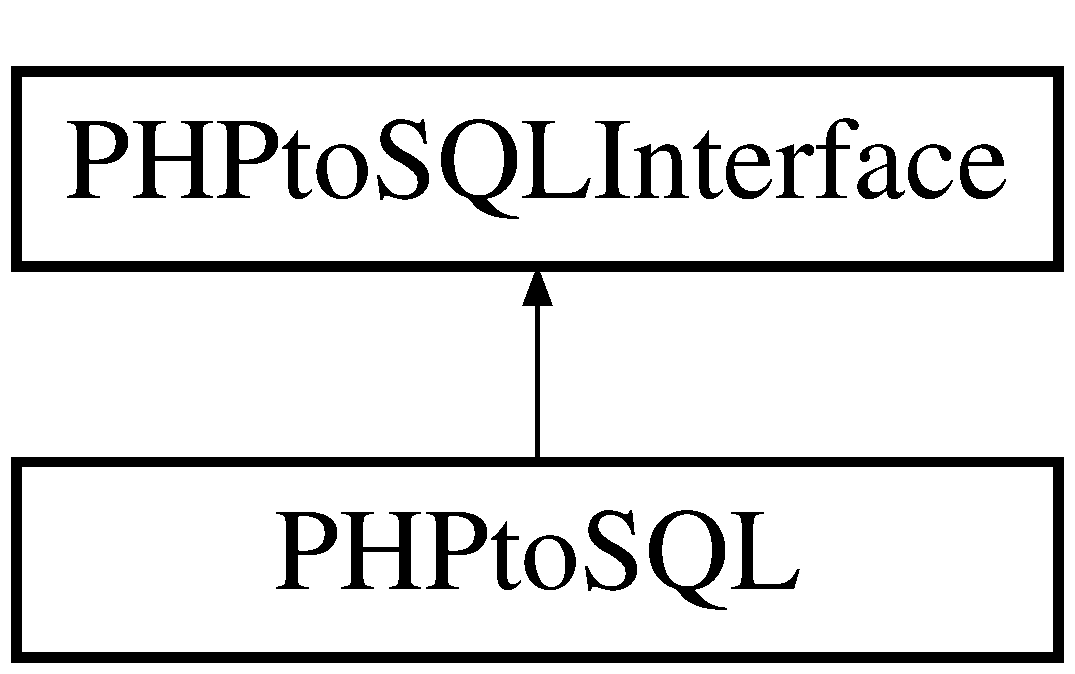
\includegraphics[height=2.000000cm]{interface_p_h_pto_s_q_l_interface}
\end{center}
\end{figure}
\subsection*{Public Member Functions}
\begin{DoxyCompactItemize}
\item 
\hyperlink{interface_p_h_pto_s_q_l_interface_a800f8efee13692788b13ee57c5960092}{\+\_\+\+\_\+construct} (\$db)
\item 
\hyperlink{interface_p_h_pto_s_q_l_interface_a421831a265621325e1fdd19aace0c758}{\+\_\+\+\_\+destruct} ()
\item 
\hyperlink{interface_p_h_pto_s_q_l_interface_a6e6deaf037e5413c56743ab1985fc0b6}{get\+Num\+Cars\+This\+Week} (\$location\+Choice)
\begin{DoxyCompactList}\small\item\em Gets the number of cars in the last week starting from today. \end{DoxyCompactList}\item 
\hyperlink{interface_p_h_pto_s_q_l_interface_a88bd9a6c7f64a8f733270a7134204ebb}{get\+Traffic\+By\+Year} (\$year, \$location\+Choice)
\begin{DoxyCompactList}\small\item\em Gives the traffic for each month in an array for the specified year passed in. \end{DoxyCompactList}\item 
\hyperlink{interface_p_h_pto_s_q_l_interface_a2389b15a72a087f39f462b1ff8f8ef95}{get\+Traffic\+By\+Month} (\$year, \$month, \$location\+Choice)
\begin{DoxyCompactList}\small\item\em Gets the traffic for each day during the specified month of the specified year. \end{DoxyCompactList}\item 
\hyperlink{interface_p_h_pto_s_q_l_interface_a6278f024da07a6ff95ffcf3efc6c0c5d}{get\+Traffic\+By\+Day} (\$year, \$month, \$day, \$location\+Choice)
\begin{DoxyCompactList}\small\item\em Gets the traffic for each hour and returns it in a 24 element array. \end{DoxyCompactList}\item 
\hyperlink{interface_p_h_pto_s_q_l_interface_ac91d0c56506620188f25007d30f1e8d0}{get\+Traffic\+Time\+Range} (\$year1, \$month1, \$day1, \$year2, \$month2, \$day2, \$location\+Choice)
\begin{DoxyCompactList}\small\item\em Takes in a date range (start and end date) and counts the number of cars in the given range. \end{DoxyCompactList}\item 
\hyperlink{interface_p_h_pto_s_q_l_interface_a64377368eb86a5a874483663c7da1407}{get\+List\+Of\+Locations} ()
\begin{DoxyCompactList}\small\item\em Will return the names of all different locations (parking lots) that are being recorded in the database. \end{DoxyCompactList}\item 
\hyperlink{interface_p_h_pto_s_q_l_interface_acc7b884d5cfc62ca661996820eebbba2}{Get\+Minimum\+Count\+In\+Hour} (\$count\+By\+Hour, \$date\+By\+Hour)
\begin{DoxyCompactList}\small\item\em Finds the minimum count for an hour in a specific time range. \end{DoxyCompactList}\item 
\hyperlink{interface_p_h_pto_s_q_l_interface_a59876f14f59f0b3321ae144eb0987692}{Get\+Median\+Count\+In\+Hour} (\$count\+By\+Hour, \$date\+By\+Hour)
\begin{DoxyCompactList}\small\item\em Finds the median count for an hour in a specific time range. \end{DoxyCompactList}\item 
\hyperlink{interface_p_h_pto_s_q_l_interface_ab4dfd011e2c8436c0284c99573d30d4a}{Get\+Maximum\+Count\+In\+Hour} (\$count\+By\+Hour, \$date\+By\+Hour)
\begin{DoxyCompactList}\small\item\em Finds the maximum count for an hour in a specific time range. \end{DoxyCompactList}\item 
\hyperlink{interface_p_h_pto_s_q_l_interface_a085d2dda8ee0aa89eba99f4b475851d1}{Get\+Average\+Count\+In\+Hour} (\$count\+By\+Hour)
\begin{DoxyCompactList}\small\item\em Finds average number of people counted during an hour in a specific time range. \end{DoxyCompactList}\item 
\hyperlink{interface_p_h_pto_s_q_l_interface_ac5a84f4e20620ec0cfac496528ce01ec}{Execute\+Query} (\$Time1, \$Time2, \$C\+O\+M\+M\+ON)
\begin{DoxyCompactList}\small\item\em A function to execute a query of correct My\+S\+QL syntax for the specified instance of the database within a certain time range. \end{DoxyCompactList}\item 
\hyperlink{interface_p_h_pto_s_q_l_interface_adbaa8f880037cb88ee1f527f6c0971b2}{Convert\+Time} (\$Time)
\begin{DoxyCompactList}\small\item\em Converts a time of a certain format to that of another. \end{DoxyCompactList}\item 
\hyperlink{interface_p_h_pto_s_q_l_interface_a01acbca2f4fed77736c1c498fb57583c}{Print\+Results} (\$results)
\begin{DoxyCompactList}\small\item\em Print\+Results is a function used to print the results of a query. \end{DoxyCompactList}\item 
\hyperlink{interface_p_h_pto_s_q_l_interface_a8fcdf2951d5159f94775133b11c29328}{Group\+Results\+By\+Hour} (\$results)
\begin{DoxyCompactList}\small\item\em Groups the results of a query by hour and counts the number of results within each hour of the time range. \end{DoxyCompactList}\item 
\hyperlink{interface_p_h_pto_s_q_l_interface_a939709f50283d3d5e8297fb0f608acf4}{Reformat\+Date} (\$date)
\begin{DoxyCompactList}\small\item\em Reformats a date into a more readable format. \end{DoxyCompactList}\end{DoxyCompactItemize}


\subsection{Detailed Description}
Created by Php\+Storm. User\+: Jabroni Date\+: 4/22/18 Time\+: 2\+:58 PM 

\subsection{Constructor \& Destructor Documentation}
\index{P\+H\+Pto\+S\+Q\+L\+Interface@{P\+H\+Pto\+S\+Q\+L\+Interface}!\+\_\+\+\_\+construct@{\+\_\+\+\_\+construct}}
\index{\+\_\+\+\_\+construct@{\+\_\+\+\_\+construct}!P\+H\+Pto\+S\+Q\+L\+Interface@{P\+H\+Pto\+S\+Q\+L\+Interface}}
\subsubsection[{\texorpdfstring{\+\_\+\+\_\+construct(\$db)}{__construct($db)}}]{\setlength{\rightskip}{0pt plus 5cm}\+\_\+\+\_\+construct (
\begin{DoxyParamCaption}
\item[{}]{\$db}
\end{DoxyParamCaption}
)}\hypertarget{interface_p_h_pto_s_q_l_interface_a800f8efee13692788b13ee57c5960092}{}\label{interface_p_h_pto_s_q_l_interface_a800f8efee13692788b13ee57c5960092}
D\+B\+A\+PI constructor. 
\begin{DoxyParams}{Parameters}
{\em \$db} & Mostly sets up the dates in this object. Also sets the timezone to our timezone. \\
\hline
\end{DoxyParams}


Implemented in \hyperlink{class_p_h_pto_s_q_l_a800f8efee13692788b13ee57c5960092}{P\+H\+Pto\+S\+QL}.

\index{P\+H\+Pto\+S\+Q\+L\+Interface@{P\+H\+Pto\+S\+Q\+L\+Interface}!\+\_\+\+\_\+destruct@{\+\_\+\+\_\+destruct}}
\index{\+\_\+\+\_\+destruct@{\+\_\+\+\_\+destruct}!P\+H\+Pto\+S\+Q\+L\+Interface@{P\+H\+Pto\+S\+Q\+L\+Interface}}
\subsubsection[{\texorpdfstring{\+\_\+\+\_\+destruct()}{__destruct()}}]{\setlength{\rightskip}{0pt plus 5cm}\+\_\+\+\_\+destruct (
\begin{DoxyParamCaption}
{}
\end{DoxyParamCaption}
)}\hypertarget{interface_p_h_pto_s_q_l_interface_a421831a265621325e1fdd19aace0c758}{}\label{interface_p_h_pto_s_q_l_interface_a421831a265621325e1fdd19aace0c758}
Class destructor 

Implemented in \hyperlink{class_p_h_pto_s_q_l_a421831a265621325e1fdd19aace0c758}{P\+H\+Pto\+S\+QL}.



\subsection{Member Function Documentation}
\index{P\+H\+Pto\+S\+Q\+L\+Interface@{P\+H\+Pto\+S\+Q\+L\+Interface}!Convert\+Time@{Convert\+Time}}
\index{Convert\+Time@{Convert\+Time}!P\+H\+Pto\+S\+Q\+L\+Interface@{P\+H\+Pto\+S\+Q\+L\+Interface}}
\subsubsection[{\texorpdfstring{Convert\+Time(\$\+Time)}{ConvertTime($Time)}}]{\setlength{\rightskip}{0pt plus 5cm}Convert\+Time (
\begin{DoxyParamCaption}
\item[{}]{\$\+Time}
\end{DoxyParamCaption}
)}\hypertarget{interface_p_h_pto_s_q_l_interface_adbaa8f880037cb88ee1f527f6c0971b2}{}\label{interface_p_h_pto_s_q_l_interface_adbaa8f880037cb88ee1f527f6c0971b2}


Converts a time of a certain format to that of another. 


\begin{DoxyParams}{Parameters}
{\em \$\+Time} & -\/ timestamp of the format ‘\+Y\+Y\+Y\+Y-\/\+M\+M-\/\+D\+D\+T\+HH\+:M\+M’. \\
\hline
\end{DoxyParams}
\begin{DoxyReturn}{Returns}
string -\/ which is of the form ‘\+Y\+Y\+Y\+Y-\/\+M\+M-\/\+DD H\+H\+:\+MM\+:00’. 
\end{DoxyReturn}


Implemented in \hyperlink{class_p_h_pto_s_q_l_adbaa8f880037cb88ee1f527f6c0971b2}{P\+H\+Pto\+S\+QL}.

\index{P\+H\+Pto\+S\+Q\+L\+Interface@{P\+H\+Pto\+S\+Q\+L\+Interface}!Execute\+Query@{Execute\+Query}}
\index{Execute\+Query@{Execute\+Query}!P\+H\+Pto\+S\+Q\+L\+Interface@{P\+H\+Pto\+S\+Q\+L\+Interface}}
\subsubsection[{\texorpdfstring{Execute\+Query(\$\+Time1, \$\+Time2, \$\+C\+O\+M\+M\+O\+N)}{ExecuteQuery($Time1, $Time2, $COMMON)}}]{\setlength{\rightskip}{0pt plus 5cm}Execute\+Query (
\begin{DoxyParamCaption}
\item[{}]{\$\+Time1, }
\item[{}]{\$\+Time2, }
\item[{}]{\$\+C\+O\+M\+M\+ON}
\end{DoxyParamCaption}
)}\hypertarget{interface_p_h_pto_s_q_l_interface_ac5a84f4e20620ec0cfac496528ce01ec}{}\label{interface_p_h_pto_s_q_l_interface_ac5a84f4e20620ec0cfac496528ce01ec}


A function to execute a query of correct My\+S\+QL syntax for the specified instance of the database within a certain time range. 


\begin{DoxyParams}{Parameters}
{\em \$\+Time1} & -\/ First timestamp of the format ‘\+Y\+Y\+Y\+Y-\/\+M\+M-\/\+DD H\+H\+:\+MM\+:00’ \\
\hline
{\em \$\+Time2} & -\/ Second timestamp of the format ‘\+Y\+Y\+Y\+Y-\/\+M\+M-\/\+DD H\+H\+:\+MM\+:00’. \\
\hline
{\em \$\+C\+O\+M\+M\+ON} & -\/ common instance that connects to the database. \\
\hline
\end{DoxyParams}
\begin{DoxyReturn}{Returns}
array -\/ all of the resulting data (in rows) returned from the query.
\end{DoxyReturn}
Usage\+: ~\newline
 \$\+Time1 = \$\+\_\+\+P\+O\+ST\mbox{[}\char`\"{}\+Time1\char`\"{}\mbox{]}; ~\newline
 \$\+Time2 = \$\+\_\+\+P\+O\+ST\mbox{[}\char`\"{}\+Time2\char`\"{}\mbox{]}; ~\newline
 // Convert input times into the correct Timestamp format ~\newline
 \$time1\+Format = Convert\+Time(\$\+Time1); ~\newline
 \$time2\+Format = Convert\+Time(\$\+Time2); ~\newline
 // Create a new \hyperlink{class_common}{Common} instance to connect to the database ~\newline
 \$debug = false; ~\newline
 \$\+C\+O\+M\+M\+ON = new \hyperlink{class_common}{Common}(\$debug); ~\newline
 // Execute query and fetch the results ~\newline
 \$results = Execute\+Query(\$time1\+Format, \$time2\+Format, \$\+C\+O\+M\+M\+ON); ~\newline
 

Implemented in \hyperlink{class_p_h_pto_s_q_l_ac5a84f4e20620ec0cfac496528ce01ec}{P\+H\+Pto\+S\+QL}.

\index{P\+H\+Pto\+S\+Q\+L\+Interface@{P\+H\+Pto\+S\+Q\+L\+Interface}!Get\+Average\+Count\+In\+Hour@{Get\+Average\+Count\+In\+Hour}}
\index{Get\+Average\+Count\+In\+Hour@{Get\+Average\+Count\+In\+Hour}!P\+H\+Pto\+S\+Q\+L\+Interface@{P\+H\+Pto\+S\+Q\+L\+Interface}}
\subsubsection[{\texorpdfstring{Get\+Average\+Count\+In\+Hour(\$count\+By\+Hour)}{GetAverageCountInHour($countByHour)}}]{\setlength{\rightskip}{0pt plus 5cm}Get\+Average\+Count\+In\+Hour (
\begin{DoxyParamCaption}
\item[{}]{\$count\+By\+Hour}
\end{DoxyParamCaption}
)}\hypertarget{interface_p_h_pto_s_q_l_interface_a085d2dda8ee0aa89eba99f4b475851d1}{}\label{interface_p_h_pto_s_q_l_interface_a085d2dda8ee0aa89eba99f4b475851d1}


Finds average number of people counted during an hour in a specific time range. 


\begin{DoxyParams}{Parameters}
{\em \$count\+By\+Hour} & -\/ the array of counts by hour returned from Group\+Results\+By\+Hour. \\
\hline
\end{DoxyParams}
\begin{DoxyReturn}{Returns}
integer -\/ Returns the average number of people recorded in an hour of the specific time range. 
\end{DoxyReturn}


Implemented in \hyperlink{class_p_h_pto_s_q_l_a085d2dda8ee0aa89eba99f4b475851d1}{P\+H\+Pto\+S\+QL}.

\index{P\+H\+Pto\+S\+Q\+L\+Interface@{P\+H\+Pto\+S\+Q\+L\+Interface}!get\+List\+Of\+Locations@{get\+List\+Of\+Locations}}
\index{get\+List\+Of\+Locations@{get\+List\+Of\+Locations}!P\+H\+Pto\+S\+Q\+L\+Interface@{P\+H\+Pto\+S\+Q\+L\+Interface}}
\subsubsection[{\texorpdfstring{get\+List\+Of\+Locations()}{getListOfLocations()}}]{\setlength{\rightskip}{0pt plus 5cm}get\+List\+Of\+Locations (
\begin{DoxyParamCaption}
{}
\end{DoxyParamCaption}
)}\hypertarget{interface_p_h_pto_s_q_l_interface_a64377368eb86a5a874483663c7da1407}{}\label{interface_p_h_pto_s_q_l_interface_a64377368eb86a5a874483663c7da1407}


Will return the names of all different locations (parking lots) that are being recorded in the database. 

\begin{DoxyReturn}{Returns}
array of strings
\end{DoxyReturn}
Usage\+: ~\newline
 \$list\+Locations\mbox{[}\mbox{]} = \hyperlink{interface_p_h_pto_s_q_l_interface_a64377368eb86a5a874483663c7da1407}{get\+List\+Of\+Locations()}; 

Implemented in \hyperlink{class_p_h_pto_s_q_l_a64377368eb86a5a874483663c7da1407}{P\+H\+Pto\+S\+QL}.

\index{P\+H\+Pto\+S\+Q\+L\+Interface@{P\+H\+Pto\+S\+Q\+L\+Interface}!Get\+Maximum\+Count\+In\+Hour@{Get\+Maximum\+Count\+In\+Hour}}
\index{Get\+Maximum\+Count\+In\+Hour@{Get\+Maximum\+Count\+In\+Hour}!P\+H\+Pto\+S\+Q\+L\+Interface@{P\+H\+Pto\+S\+Q\+L\+Interface}}
\subsubsection[{\texorpdfstring{Get\+Maximum\+Count\+In\+Hour(\$count\+By\+Hour, \$date\+By\+Hour)}{GetMaximumCountInHour($countByHour, $dateByHour)}}]{\setlength{\rightskip}{0pt plus 5cm}Get\+Maximum\+Count\+In\+Hour (
\begin{DoxyParamCaption}
\item[{}]{\$count\+By\+Hour, }
\item[{}]{\$date\+By\+Hour}
\end{DoxyParamCaption}
)}\hypertarget{interface_p_h_pto_s_q_l_interface_ab4dfd011e2c8436c0284c99573d30d4a}{}\label{interface_p_h_pto_s_q_l_interface_ab4dfd011e2c8436c0284c99573d30d4a}


Finds the maximum count for an hour in a specific time range. 


\begin{DoxyParams}{Parameters}
{\em \$count\+By\+Hour} & -\/ the array of counts by hour returned from Group\+Results\+By\+Hour. \\
\hline
{\em \$date\+By\+Hour} & -\/ the corresponding array of dates sorted by hour returned from Group\+Results\+By\+Hour. \\
\hline
\end{DoxyParams}
\begin{DoxyReturn}{Returns}
2 arrays -\/ Returns an array containing (1) the maximum count within an hour and (2) the corresponding time for which the count was recorded. 
\end{DoxyReturn}


Implemented in \hyperlink{class_p_h_pto_s_q_l_ab4dfd011e2c8436c0284c99573d30d4a}{P\+H\+Pto\+S\+QL}.

\index{P\+H\+Pto\+S\+Q\+L\+Interface@{P\+H\+Pto\+S\+Q\+L\+Interface}!Get\+Median\+Count\+In\+Hour@{Get\+Median\+Count\+In\+Hour}}
\index{Get\+Median\+Count\+In\+Hour@{Get\+Median\+Count\+In\+Hour}!P\+H\+Pto\+S\+Q\+L\+Interface@{P\+H\+Pto\+S\+Q\+L\+Interface}}
\subsubsection[{\texorpdfstring{Get\+Median\+Count\+In\+Hour(\$count\+By\+Hour, \$date\+By\+Hour)}{GetMedianCountInHour($countByHour, $dateByHour)}}]{\setlength{\rightskip}{0pt plus 5cm}Get\+Median\+Count\+In\+Hour (
\begin{DoxyParamCaption}
\item[{}]{\$count\+By\+Hour, }
\item[{}]{\$date\+By\+Hour}
\end{DoxyParamCaption}
)}\hypertarget{interface_p_h_pto_s_q_l_interface_a59876f14f59f0b3321ae144eb0987692}{}\label{interface_p_h_pto_s_q_l_interface_a59876f14f59f0b3321ae144eb0987692}


Finds the median count for an hour in a specific time range. 


\begin{DoxyParams}{Parameters}
{\em \$count\+By\+Hour} & -\/ the array of counts by hour returned from Group\+Results\+By\+Hour. \\
\hline
{\em \$date\+By\+Hour} & -\/ the corresponding array of dates sorted by hour returned from Group\+Results\+By\+Hour. \\
\hline
\end{DoxyParams}
\begin{DoxyReturn}{Returns}
array -\/ Returns an array containing (1) the median count within an hour and (2) the corresponding time for which the count was recorded. 
\end{DoxyReturn}


Implemented in \hyperlink{class_p_h_pto_s_q_l_a59876f14f59f0b3321ae144eb0987692}{P\+H\+Pto\+S\+QL}.

\index{P\+H\+Pto\+S\+Q\+L\+Interface@{P\+H\+Pto\+S\+Q\+L\+Interface}!Get\+Minimum\+Count\+In\+Hour@{Get\+Minimum\+Count\+In\+Hour}}
\index{Get\+Minimum\+Count\+In\+Hour@{Get\+Minimum\+Count\+In\+Hour}!P\+H\+Pto\+S\+Q\+L\+Interface@{P\+H\+Pto\+S\+Q\+L\+Interface}}
\subsubsection[{\texorpdfstring{Get\+Minimum\+Count\+In\+Hour(\$count\+By\+Hour, \$date\+By\+Hour)}{GetMinimumCountInHour($countByHour, $dateByHour)}}]{\setlength{\rightskip}{0pt plus 5cm}Get\+Minimum\+Count\+In\+Hour (
\begin{DoxyParamCaption}
\item[{}]{\$count\+By\+Hour, }
\item[{}]{\$date\+By\+Hour}
\end{DoxyParamCaption}
)}\hypertarget{interface_p_h_pto_s_q_l_interface_acc7b884d5cfc62ca661996820eebbba2}{}\label{interface_p_h_pto_s_q_l_interface_acc7b884d5cfc62ca661996820eebbba2}


Finds the minimum count for an hour in a specific time range. 


\begin{DoxyParams}{Parameters}
{\em \$count\+By\+Hour} & -\/ the corresponding array of dates sorted by hour returned from Group\+Results\+By\+Hour. \\
\hline
{\em \$date\+By\+Hour} & -\/ the array of counts by hour returned from Group\+Results\+By\+Hour. \\
\hline
\end{DoxyParams}
\begin{DoxyReturn}{Returns}
Returns an array containing (1) the minimum count within an hour and (2) the corresponding time for which the count was recorded. 
\end{DoxyReturn}


Implemented in \hyperlink{class_p_h_pto_s_q_l_acc7b884d5cfc62ca661996820eebbba2}{P\+H\+Pto\+S\+QL}.

\index{P\+H\+Pto\+S\+Q\+L\+Interface@{P\+H\+Pto\+S\+Q\+L\+Interface}!get\+Num\+Cars\+This\+Week@{get\+Num\+Cars\+This\+Week}}
\index{get\+Num\+Cars\+This\+Week@{get\+Num\+Cars\+This\+Week}!P\+H\+Pto\+S\+Q\+L\+Interface@{P\+H\+Pto\+S\+Q\+L\+Interface}}
\subsubsection[{\texorpdfstring{get\+Num\+Cars\+This\+Week(\$location\+Choice)}{getNumCarsThisWeek($locationChoice)}}]{\setlength{\rightskip}{0pt plus 5cm}get\+Num\+Cars\+This\+Week (
\begin{DoxyParamCaption}
\item[{}]{\$location\+Choice}
\end{DoxyParamCaption}
)}\hypertarget{interface_p_h_pto_s_q_l_interface_a6e6deaf037e5413c56743ab1985fc0b6}{}\label{interface_p_h_pto_s_q_l_interface_a6e6deaf037e5413c56743ab1985fc0b6}


Gets the number of cars in the last week starting from today. 

\begin{DoxyReturn}{Returns}
int
\end{DoxyReturn}
Usage\+: ~\newline
 \$num\+Cars = get\+Num\+Cars\+This\+Week(\char`\"{}lot35\char`\"{}); for Lot 35 

Implemented in \hyperlink{class_p_h_pto_s_q_l_a6e6deaf037e5413c56743ab1985fc0b6}{P\+H\+Pto\+S\+QL}.

\index{P\+H\+Pto\+S\+Q\+L\+Interface@{P\+H\+Pto\+S\+Q\+L\+Interface}!get\+Traffic\+By\+Day@{get\+Traffic\+By\+Day}}
\index{get\+Traffic\+By\+Day@{get\+Traffic\+By\+Day}!P\+H\+Pto\+S\+Q\+L\+Interface@{P\+H\+Pto\+S\+Q\+L\+Interface}}
\subsubsection[{\texorpdfstring{get\+Traffic\+By\+Day(\$year, \$month, \$day, \$location\+Choice)}{getTrafficByDay($year, $month, $day, $locationChoice)}}]{\setlength{\rightskip}{0pt plus 5cm}get\+Traffic\+By\+Day (
\begin{DoxyParamCaption}
\item[{}]{\$year, }
\item[{}]{\$month, }
\item[{}]{\$day, }
\item[{}]{\$location\+Choice}
\end{DoxyParamCaption}
)}\hypertarget{interface_p_h_pto_s_q_l_interface_a6278f024da07a6ff95ffcf3efc6c0c5d}{}\label{interface_p_h_pto_s_q_l_interface_a6278f024da07a6ff95ffcf3efc6c0c5d}


Gets the traffic for each hour and returns it in a 24 element array. 


\begin{DoxyParams}{Parameters}
{\em \$year} & \\
\hline
{\em \$month} & \\
\hline
{\em \$day} & \\
\hline
{\em \$location\+Choice} & \\
\hline
\end{DoxyParams}
\begin{DoxyReturn}{Returns}
int array -\/ length 24 array with the traffic number for each our of the day
\end{DoxyReturn}
Usage\+: ~\newline
 $<$ \$day\+Array = get\+Traffic\+By\+Day(2018, 2, 15, \char`\"{}lot35\char`\"{});$>$ for Febraury 15, 2018 for Lot 35 

Implemented in \hyperlink{class_p_h_pto_s_q_l_a6278f024da07a6ff95ffcf3efc6c0c5d}{P\+H\+Pto\+S\+QL}.

\index{P\+H\+Pto\+S\+Q\+L\+Interface@{P\+H\+Pto\+S\+Q\+L\+Interface}!get\+Traffic\+By\+Month@{get\+Traffic\+By\+Month}}
\index{get\+Traffic\+By\+Month@{get\+Traffic\+By\+Month}!P\+H\+Pto\+S\+Q\+L\+Interface@{P\+H\+Pto\+S\+Q\+L\+Interface}}
\subsubsection[{\texorpdfstring{get\+Traffic\+By\+Month(\$year, \$month, \$location\+Choice)}{getTrafficByMonth($year, $month, $locationChoice)}}]{\setlength{\rightskip}{0pt plus 5cm}get\+Traffic\+By\+Month (
\begin{DoxyParamCaption}
\item[{}]{\$year, }
\item[{}]{\$month, }
\item[{}]{\$location\+Choice}
\end{DoxyParamCaption}
)}\hypertarget{interface_p_h_pto_s_q_l_interface_a2389b15a72a087f39f462b1ff8f8ef95}{}\label{interface_p_h_pto_s_q_l_interface_a2389b15a72a087f39f462b1ff8f8ef95}


Gets the traffic for each day during the specified month of the specified year. 


\begin{DoxyParams}{Parameters}
{\em \$year} & \\
\hline
{\em \$month} & \\
\hline
{\em \$location\+Choice} & \\
\hline
\end{DoxyParams}
\begin{DoxyReturn}{Returns}
int array -\/ array with the traffic number for each day of the specified month
\end{DoxyReturn}
Usage\+: ~\newline
 \$month\+Array = get\+Traffic\+By\+Month(2018, 2, \char`\"{}lot35\char`\"{}); // for February 2018 for Lot 35 

Implemented in \hyperlink{class_p_h_pto_s_q_l_a2389b15a72a087f39f462b1ff8f8ef95}{P\+H\+Pto\+S\+QL}.

\index{P\+H\+Pto\+S\+Q\+L\+Interface@{P\+H\+Pto\+S\+Q\+L\+Interface}!get\+Traffic\+By\+Year@{get\+Traffic\+By\+Year}}
\index{get\+Traffic\+By\+Year@{get\+Traffic\+By\+Year}!P\+H\+Pto\+S\+Q\+L\+Interface@{P\+H\+Pto\+S\+Q\+L\+Interface}}
\subsubsection[{\texorpdfstring{get\+Traffic\+By\+Year(\$year, \$location\+Choice)}{getTrafficByYear($year, $locationChoice)}}]{\setlength{\rightskip}{0pt plus 5cm}get\+Traffic\+By\+Year (
\begin{DoxyParamCaption}
\item[{}]{\$year, }
\item[{}]{\$location\+Choice}
\end{DoxyParamCaption}
)}\hypertarget{interface_p_h_pto_s_q_l_interface_a88bd9a6c7f64a8f733270a7134204ebb}{}\label{interface_p_h_pto_s_q_l_interface_a88bd9a6c7f64a8f733270a7134204ebb}


Gives the traffic for each month in an array for the specified year passed in. 


\begin{DoxyParams}{Parameters}
{\em \$year} & \\
\hline
{\em \$location\+Choice} & -\/ string for the lot you want to put in \\
\hline
\end{DoxyParams}
\begin{DoxyReturn}{Returns}
int array -\/ a length 12 array where each element is the number of cars that passed through for that month. If there were 8 cars that passed through in April, the element at index 3 would be 8
\end{DoxyReturn}
Usage\+: ~\newline
 \$year\+Array = get\+Traffic\+By\+Year(2018, \char`\"{}lot35\char`\"{}); for 2018 for Lot 35 

Implemented in \hyperlink{class_p_h_pto_s_q_l_a88bd9a6c7f64a8f733270a7134204ebb}{P\+H\+Pto\+S\+QL}.

\index{P\+H\+Pto\+S\+Q\+L\+Interface@{P\+H\+Pto\+S\+Q\+L\+Interface}!get\+Traffic\+Time\+Range@{get\+Traffic\+Time\+Range}}
\index{get\+Traffic\+Time\+Range@{get\+Traffic\+Time\+Range}!P\+H\+Pto\+S\+Q\+L\+Interface@{P\+H\+Pto\+S\+Q\+L\+Interface}}
\subsubsection[{\texorpdfstring{get\+Traffic\+Time\+Range(\$year1, \$month1, \$day1, \$year2, \$month2, \$day2, \$location\+Choice)}{getTrafficTimeRange($year1, $month1, $day1, $year2, $month2, $day2, $locationChoice)}}]{\setlength{\rightskip}{0pt plus 5cm}get\+Traffic\+Time\+Range (
\begin{DoxyParamCaption}
\item[{}]{\$year1, }
\item[{}]{\$month1, }
\item[{}]{\$day1, }
\item[{}]{\$year2, }
\item[{}]{\$month2, }
\item[{}]{\$day2, }
\item[{}]{\$location\+Choice}
\end{DoxyParamCaption}
)}\hypertarget{interface_p_h_pto_s_q_l_interface_ac91d0c56506620188f25007d30f1e8d0}{}\label{interface_p_h_pto_s_q_l_interface_ac91d0c56506620188f25007d30f1e8d0}


Takes in a date range (start and end date) and counts the number of cars in the given range. 


\begin{DoxyParams}{Parameters}
{\em \$year1} & \\
\hline
{\em \$month1} & \\
\hline
{\em \$day1} & \\
\hline
{\em \$year2} & \\
\hline
{\em \$month2} & \\
\hline
{\em \$day2} & \\
\hline
{\em \$location\+Choice} & \\
\hline
\end{DoxyParams}
\begin{DoxyReturn}{Returns}
integer -\/ the number of cars in the time range
\end{DoxyReturn}
Usage\+: ~\newline
 \$traffic\+In\+Range = get\+Traffic\+Time\+Range(2018, 2, 15, 2018, 2, 28, \char`\"{}lot35\char`\"{}); ~\newline
 for number of cars between 2/15/2018 and 2/28/2018 for Lot 35 

Implemented in \hyperlink{class_p_h_pto_s_q_l_ac91d0c56506620188f25007d30f1e8d0}{P\+H\+Pto\+S\+QL}.

\index{P\+H\+Pto\+S\+Q\+L\+Interface@{P\+H\+Pto\+S\+Q\+L\+Interface}!Group\+Results\+By\+Hour@{Group\+Results\+By\+Hour}}
\index{Group\+Results\+By\+Hour@{Group\+Results\+By\+Hour}!P\+H\+Pto\+S\+Q\+L\+Interface@{P\+H\+Pto\+S\+Q\+L\+Interface}}
\subsubsection[{\texorpdfstring{Group\+Results\+By\+Hour(\$results)}{GroupResultsByHour($results)}}]{\setlength{\rightskip}{0pt plus 5cm}Group\+Results\+By\+Hour (
\begin{DoxyParamCaption}
\item[{}]{\$results}
\end{DoxyParamCaption}
)}\hypertarget{interface_p_h_pto_s_q_l_interface_a8fcdf2951d5159f94775133b11c29328}{}\label{interface_p_h_pto_s_q_l_interface_a8fcdf2951d5159f94775133b11c29328}


Groups the results of a query by hour and counts the number of results within each hour of the time range. 


\begin{DoxyParams}{Parameters}
{\em \$results} & -\/ the results returned from a query, specifically from the function, \hyperlink{interface_p_h_pto_s_q_l_interface_ac5a84f4e20620ec0cfac496528ce01ec}{Execute\+Query()}. \\
\hline
\end{DoxyParams}
\begin{DoxyReturn}{Returns}
array -\/ Returns an array containing (1) an array of the dates within the results, grouped by hour, and (2) an array containing the counts for each corresponding hour of the dates array. 
\end{DoxyReturn}


Implemented in \hyperlink{class_p_h_pto_s_q_l_a8fcdf2951d5159f94775133b11c29328}{P\+H\+Pto\+S\+QL}.

\index{P\+H\+Pto\+S\+Q\+L\+Interface@{P\+H\+Pto\+S\+Q\+L\+Interface}!Print\+Results@{Print\+Results}}
\index{Print\+Results@{Print\+Results}!P\+H\+Pto\+S\+Q\+L\+Interface@{P\+H\+Pto\+S\+Q\+L\+Interface}}
\subsubsection[{\texorpdfstring{Print\+Results(\$results)}{PrintResults($results)}}]{\setlength{\rightskip}{0pt plus 5cm}Print\+Results (
\begin{DoxyParamCaption}
\item[{}]{\$results}
\end{DoxyParamCaption}
)}\hypertarget{interface_p_h_pto_s_q_l_interface_a01acbca2f4fed77736c1c498fb57583c}{}\label{interface_p_h_pto_s_q_l_interface_a01acbca2f4fed77736c1c498fb57583c}


Print\+Results is a function used to print the results of a query. 


\begin{DoxyParams}{Parameters}
{\em \$results} & -\/ the results returned from a query, specifically from the function, \hyperlink{interface_p_h_pto_s_q_l_interface_ac5a84f4e20620ec0cfac496528ce01ec}{Execute\+Query()} \\
\hline
\end{DoxyParams}
\begin{DoxyReturn}{Returns}
void -\/ returns echo’s html code to return rows with an entry number and the timestamp for it 
\end{DoxyReturn}


Implemented in \hyperlink{class_p_h_pto_s_q_l_a01acbca2f4fed77736c1c498fb57583c}{P\+H\+Pto\+S\+QL}.

\index{P\+H\+Pto\+S\+Q\+L\+Interface@{P\+H\+Pto\+S\+Q\+L\+Interface}!Reformat\+Date@{Reformat\+Date}}
\index{Reformat\+Date@{Reformat\+Date}!P\+H\+Pto\+S\+Q\+L\+Interface@{P\+H\+Pto\+S\+Q\+L\+Interface}}
\subsubsection[{\texorpdfstring{Reformat\+Date(\$date)}{ReformatDate($date)}}]{\setlength{\rightskip}{0pt plus 5cm}Reformat\+Date (
\begin{DoxyParamCaption}
\item[{}]{\$date}
\end{DoxyParamCaption}
)}\hypertarget{interface_p_h_pto_s_q_l_interface_a939709f50283d3d5e8297fb0f608acf4}{}\label{interface_p_h_pto_s_q_l_interface_a939709f50283d3d5e8297fb0f608acf4}


Reformats a date into a more readable format. 


\begin{DoxyParams}{Parameters}
{\em \$date} & -\/ A date in format \char`\"{}\+Y\+Y\+Y\+Y-\/\+M\+M-\/\+D\+D H\+H\char`\"{} where HH ranges from 00 to 23. \\
\hline
\end{DoxyParams}
\begin{DoxyReturn}{Returns}
string -\/ The date in format \char`\"{}\+Y\+Y\+Y\+Y-\/\+M\+M-\/\+D\+D H\+H\+:00\char`\"{} where HH ranges from 00 to 12 A\+M/\+PM. 
\end{DoxyReturn}


Implemented in \hyperlink{class_p_h_pto_s_q_l_a939709f50283d3d5e8297fb0f608acf4}{P\+H\+Pto\+S\+QL}.



The documentation for this interface was generated from the following file\+:\begin{DoxyCompactItemize}
\item 
P\+H\+P Server Code/P\+H\+Pto\+S\+Q\+L\+Interface.\+php\end{DoxyCompactItemize}

%--- End generated contents ---

% Index
\backmatter
\newpage
\phantomsection
\clearemptydoublepage
\addcontentsline{toc}{chapter}{Index}
\printindex

\end{document}
